\documentclass[a4paper,12pt]{article}

\usepackage[utf8]{inputenc}
\usepackage[english,russian]{babel}

\usepackage[nottoc,numbib]{tocbibind} %for adding bibliography to 
                                      %table of content

\usepackage{color}   %May be necessary if you want to color links
\usepackage{hyperref}
\hypersetup{
    colorlinks=true, %set true if you want colored links
    linktoc=all,     %set to all if you want both sections and subsections linked
    linkcolor=black, %choose some color if you want links to stand out
    citecolor=black,
}

\addto\captionsrussian{\renewcommand{\refname}{Источники}}
\setlength{\parindent}{0em}
\setlength{\parskip}{1em}

\usepackage{graphicx}
\graphicspath{ {./../img/} }

\usepackage[font=small,labelfont=bf]{caption}

\begin{document}

\title{Самоорганизующаяся карта Кохонена}
\author{Козырев Сергей, 331 группа}
\maketitle

\newpage
\tableofcontents

\newpage
\section{Описание}

Самоорганизующаяся карта Кохонена - нейронная сеть с обучением без учителя, выполняющая задачу визуализации и кластеризации.\cite{wikipedia_map_ru}

Важным отличием алгоритма SOM является то, что в нем все нейроны (узлы, центры классов...) упорядочены в некоторую структуру (обычно двумерную сетку). При этом в ходе обучения модифицируется не только нейрон-победитель, но и его соседи, но в меньшей степени. За счет этого SOM можно считать одним из методов проецирования многомерного пространства в пространство с более низкой размерностью. При использовании этого алгоритма вектора, схожие в исходном пространстве, оказываются рядом и на полученной карте.\cite{basegroup}

\begin{figure}[h]
  \centering
  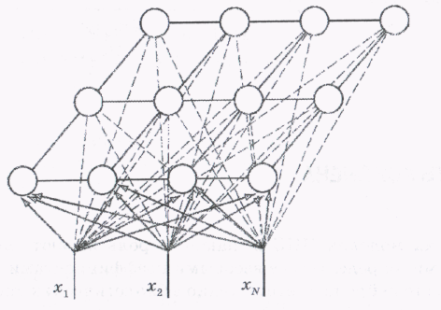
\includegraphics[width=0.5\textwidth]{structure.png}
  \caption{Структура сети, нейроны составляют двумерную сетку}
\end{figure}

\section{История}

Эту нейронную сеть предложил финский профессор Теуво Кохонен в 1980-х годах. Самоорганизующаяся карта Кохонена (SOM) выросла из ранних моделей нейронных сетей, особенно моделей ассоциативной памяти и адаптивного обучения (ср. Кохонен 1984). Новый стимул состоял в том, чтобы объяснить пространственную организацию функций мозга, особенно наблюдаемую в коре больших полушарий. Тем не менее, SOM не была первым шагом в этом направлении: следует упомянуть, по крайней мере, пространственно упорядоченные линейные детекторы фон дер Мальсбурга (1973) и модель нейронного поля Амари (1980).

Первой областью применения SOM было распознавание речи (см. рис. \ref{fig:phonemesom}). В своей абстрактной форме SOM получила широкое распространение в области анализа и исследования данных (Kaski et al. 1998, Oja et al. 2003, Pöllä et al. 2007).\cite{scholarpedia}

\begin{figure}[h]
  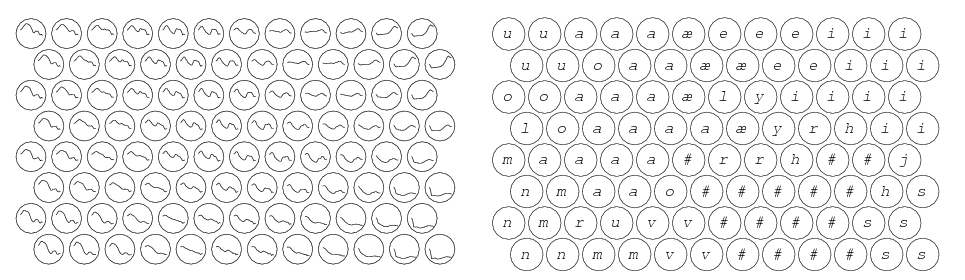
\includegraphics[width=\textwidth]{Phonemesom.png}
  \caption{Левое изображение: модели акустических спектров финских фонем, организованных на некотором расстоянии.
  Правое изображение: калибровка моделей по фонемным классам. Символ \# обозначает взрывные согласные /k, p, t/.}
  \centering
  \label{fig:phonemesom}
\end{figure}

\section{Нейронные сети Кохонена}

Нейронные сети Кохонена — более широкий класс нейронных сетей, основным элементом которых является слой Кохонена. Слой Кохонена состоит из адаптивных линейных сумматоров («линейных формальных нейронов»). Как правило, выходные сигналы слоя Кохонена обрабатываются по правилу «Победитель получает всё»: наибольший сигнал превращается в единичный, остальные обращаются в ноль.

\subsection{Слой Кохонена}

Слой Кохонена состоит из некоторого количества $n$ параллельно действующих линейных элементов. Все они имеют одинаковое число входов $m$ и получают на свои входы один и тот же вектор входных сигналов $x=(x_{1},...x_{m})$. На выходе $j$-го линейного элемента получаем сигнал 
\[
  y_{j}=w_{{j0}}+\sum _{{i=1}}^{m}w_{{ji}}x_{i},
\]
где:
\begin{itemize}
  \setlength\itemsep{0em}
  \item $w_{{ji}}$ — весовой коэффициент $i$-го входа $j$-го нейрона;
  \item $i$ — номер входа;
  \item $j$ — номер нейрона;
  \item $w_{{j0}}$ — пороговый коэффициент.
\end{itemize}

После прохождения слоя линейных элементов сигналы посылаются на обработку по правилу «победитель забирает всё»: среди выходных сигналов выполняется поиск максимального \(y_{j}\); его номер \(j_{{\max }}={{\rm {arg}}}\max _{{j}}\{y_{j}\}\). Окончательно, на выходе сигнал с номером \(j_{{\max }}\) равен единице, остальные — нулю. Если максимум одновременно достигается для нескольких \(j_{{\max }}\), то:
\begin{itemize}
  \setlength\itemsep{0em}
  \item либо принимают все соответствующие сигналы равными единице;
  \item либо равным единице принимают только первый сигнал в списке (по соглашению).
\end{itemize}

\subsection{Геометрическая интерпретация}

Большое распространение получили слои Кохонена, построенные следующим образом: каждому ($j$-му) нейрону сопоставляется точка $W_{j}=(w_{{j1}},...w_{{jm}})$ в $m$-мерном пространстве (пространстве сигналов). Для входного вектора $x=(x_{1},...x_{m})$ вычисляются его евклидовы расстояния $\rho _{j}(x)$ до точек $W_j$ и «ближайший получает всё» — тот нейрон, для которого это расстояние минимально, выдаёт единицу, остальные — нули. Следует заметить, что для сравнения расстояний достаточно вычислять линейную функцию сигнала:
\[
  \rho _{j}(x)^{2}=\|x-W_{j}\|^{2}=\|W_{j}\|^{2}-2\sum _{{i=1}}^{m}w_{{ji}}x_{i}+\|x\|^{2}
\]
(здесь $\|y\|$ — Евклидова длина вектора: $\|y\|^{2}=\sum _{i}y_{i}^{2}$). Последнее слагаемое $\|x\|^{2}$ одинаково для всех нейронов, поэтому для нахождения ближайшей точки оно не нужно. Задача сводится к поиску номера наибольшего из значений линейных функций:
\[
  j_{\max }={\rm {arg}}\max _{j}\left\{\sum _{i=1}^{m}w_{ji}x_{i}-{\frac {1}{2}}\|W_{j}\|^{2}\right\}
\]

Таким образом, координаты точки ${\displaystyle W_{j}=(w_{j1},...w_{jm})}$ совпадают с весами линейного нейрона слоя Кохонена (при этом значение порогового коэффициента ${\displaystyle w_{j0}=-\|W_{j}\|^{2}/2}$.

Если заданы точки $W_{j}=(w_{{j1}},...w_{{jm}})$, то $m$-мерное пространство разбивается на соответствующие многогранники Вороного-Дирихле $V_{j}$: многогранник $V_{j}$ состоит из точек, которые ближе к $W_j$, чем к другим $W_{k}$ ($k\neq j$).
\cite{wikipedia_network}

\section{Алгоритм обучения}
\begin{enumerate}
  \item инициализируем веса нейронов
  \item берём случайный вектор $D(t)$ из множества входных данных ($t$ - индекс вектора в массиве входных данных), находим ближайший к нему нейрон (best matching unit, BMU), пусть u - его индекс
  \item изменяем веса нейронов по формуле:
  \[
    W_v(s + 1)=W_v(s)+\theta(u, v, s) \cdot \alpha(s) \cdot (D(t) - W_v(s)),
  \]
  где:
  \begin{itemize}
    \setlength\itemsep{0em}
    \item $W_v(s)$ - вес нейрона $W_v$ на итерации $s$.
    \item $\theta(u, v, s)$ - расстояние между нейронами $W_u$ и $W_v$. Обычно используется один из двух вариантов: либо функция Гаусса, либо же расстояние до соседей равно 1, а до остальных нейронов оно приравнивается 0.
    \item $\alpha(s)$ - шаг обучения, убывающая функция.
  \end{itemize}
  \item повторяем c шага 2, пока $s < k$.\cite{algorithm}
\end{enumerate}

\section{Методы представления}

\subsection{U-matrix}
Унифицированная матрица расстояний(unified distance matrix, U-matrix) - один из способов представления получившейся карты. Карта раскрашивается в зависимости от расстояния между соседними нейронами.\cite{u_matrix}

\begin{figure}[h]
  \centering
  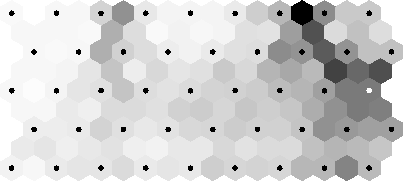
\includegraphics[width=0.8\textwidth]{u-matrix.png}
  \caption{Пример U-matrix. Чёрные точки обозначают нейроны, чем больше расстояние между соседними нейронами, тем темнее ячейки, находящиеся между ними.}
\end{figure}

\subsection{Карта входов нейронов}

Карта входов нейронов строится для каждого входа ($x_i$), где нейроны раскрашиваются в соответствии с весом $w_i$, соответствующим этому входу. Пример можно увидеть на рис. \ref{img:congress}, где все карты, кроме первых трёх, являются картами входов.

\begin{figure}[h]
  \centering
  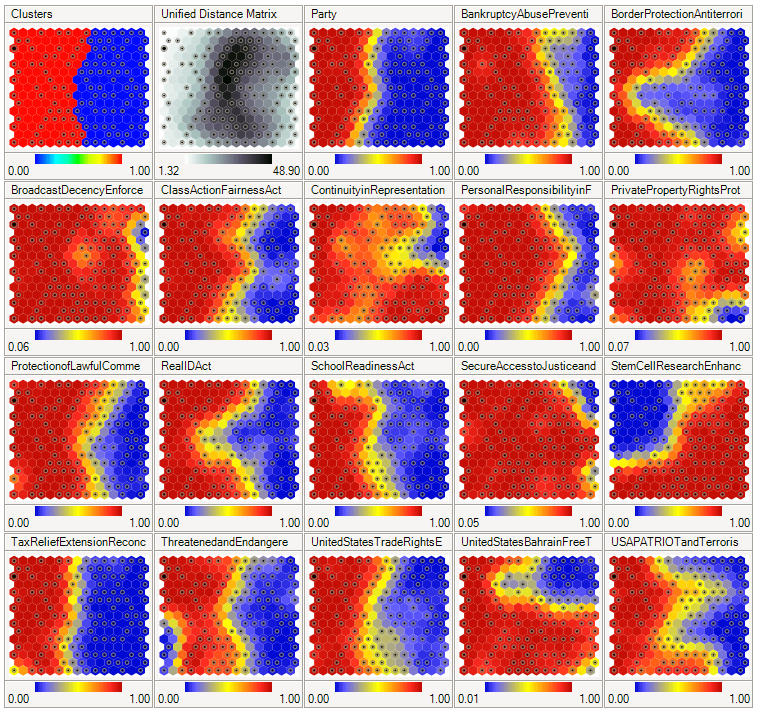
\includegraphics[width=0.5\textwidth]{congress.png}
  \caption{Самоорганизующаяся карта, показывающая схему голосования в Конгрессе США. Исходные данные представляли собой таблицу со строкой для каждого члена Конгресса и столбцами для определенных голосов, содержащими голос каждого члена " да " / " нет " / "воздержался". Алгоритм SOM расположил эти элементы в двумерной сетке, расположив подобные элементы ближе друг к другу. Первый график показывает группировку, когда данные разделены на два кластера. Второй график показывает среднее расстояние до соседей: большие расстояния темнее. Третий график предсказывает членство в Республиканской (красной) или Демократической (синей) партии. Остальные графики являются картами по одному из входов(карта входов нейронов): красный цвет означает предсказанный голос "да" по этому законопроекту, синий - голос "нет".\cite{wikipedia_map_en}}
  \label{img:congress}
\end{figure}

\subsection{Карта выходов нейронов}

На карту выходов нейронов проецируется взаимное расположение исследуемых входных данных.

\subsection{Специальные карты}

Это карта кластеров, матрица расстояний, матрица плотности попадания и другие карты, которые характеризуют кластеры, полученные в результате обучения сети Кохонена. Примером служат первые две карты из рис. \ref{img:congress}

Важно понимать, что между всеми рассмотренными картами существует взаимосвязь - все они являются разными раскрасками одних и тех же нейронов. Каждый пример из обучающей выборки имеет одно и то же расположение на всех картах.\cite{intuit}

\section{Применение}

Самоорганизующиеся карты могут использоваться для решения таких задач, как моделирование, прогнозирование, поиск закономерностей в больших массивах данных, выявление наборов независимых признаков и сжатие информации.\cite{intuit}

\begin{thebibliography}{9}
  \bibitem{scholarpedia}
    Teuvo Kohonen and Timo Honkela (2007)
    \href{http://www.scholarpedia.org/article/Kohonen_network}{Kohonen network}.
    \href{http://www.scholarpedia.org/}{Scholarpedia},
    2(1):1568.

  \bibitem{wikipedia_network}
    \href{https://ru.wikipedia.org/wiki/\%D0\%9D\%D0\%B5\%D0\%B9\%D1\%80\%D0\%BE\%D0\%BD\%D0\%BD\%D0\%B0\%D1\%8F\_\%D1\%81\%D0\%B5\%D1\%82\%D1\%8C\_\%D0\%9A\%D0\%BE\%D1\%85\%D0\%BE\%D0\%BD\%D0\%B5\%D0\%BD\%D0\%B0}
    {https://ru.wikipedia.org/wiki/Нейронная\_сеть\_Кохонена}

  \bibitem{wikipedia_map_ru}
    \href{https://ru.wikipedia.org/wiki/\%D0\%A1\%D0\%B0\%D0\%BC\%D0\%BE\%D0\%BE\%D1\%80\%D0\%B3\%D0\%B0\%D0\%BD\%D0\%B8\%D0\%B7\%D1\%83\%D1\%8E\%D1\%89\%D0\%B0\%D1\%8F\%D1\%81\%D1\%8F_\%D0\%BA\%D0\%B0\%D1\%80\%D1\%82\%D0\%B0_\%D0\%9A\%D0\%BE\%D1\%85\%D0\%BE\%D0\%BD\%D0\%B5\%D0\%BD\%D0\%B0}
    {https://ru.wikipedia.org/wiki/Самоорганизующаяся\_карта\_Кохонена}

  \bibitem{wikipedia_map_en}
    \href{https://en.wikipedia.org/wiki/Self-organizing\_map}{https://en.wikipedia.org/wiki/Self-organizing\_map}

  \bibitem{algorithm}
    \href{https://en.wikipedia.org/wiki/Self-organizing\_map\#Algorithm}
    {https://en.wikipedia.org/wiki/Self-organizing\_map\#Algorithm}

  \bibitem{basegroup}
    \href{https://basegroup.ru/community/articles/som}{https://basegroup.ru/community/articles/som}

  \bibitem{intuit}
    \href{https://www.intuit.ru/studies/courses/6/6/lecture/180?page=3}{https://www.intuit.ru/studies/courses/6/6/lecture/180?page=3}
  
  \bibitem{u_matrix}
    \href{https://users.ics.aalto.fi/jhollmen/dippa/node24.html}{https://users.ics.aalto.fi/jhollmen/dippa/node24.html}
\end{thebibliography}

\end{document}